\documentclass{article}
% \documentclass[UTF8]{ctexart}
\usepackage{amsmath,amssymb,amsfonts}  % For math symbols and fonts
\usepackage{graphicx}                   % For including images
\usepackage{hyperref}                   % For hyperlinks
\usepackage{cite}                       % For citations
% \usepackage[UTF8]{ctex}  % 注意,不是 \documentclass[UTF8]{ctexart}
% \renewcommand{\contentsname}{Contents}
% \renewcommand{\refname}{References}
% \renewcommand{\abstractname}{Abstract}

\usepackage{algorithm}
\usepackage{algorithmic}
\usepackage{array}

\usepackage{amsthm}
% Define new theorem-like environments
% Define environments
\theoremstyle{definition} % Non-italicized style
\newtheorem{definition}{Definition}[section]
\newtheorem{exercise}{Exercise}[section]

% Title and author info
\title{Wavelet Transform for Image Processing}
\author{
Zhang Jinrui\thanks{alternative email:zhangjr1022@mails.jlu.edu.cn} \\ \texttt{jerryzhang40@gmail.com}
}

\date{20250728}  % Empty date; optional, you can also specify a date here

\begin{document}

\maketitle

\begin{abstract}
    In this article, I tried to use
    Wavelet Transform to compress
    images\cite{raissi2017physics}.
\end{abstract}


\section{Decomposition \& Mother Wavelet}
A mother wavelet \(\psi\) satisfied
following property.
\(\langle\psi,\psi\rangle=1\)

And the family of the Hilbert Basis
wavelets are as follow.
\[
    \psi_{j,k}=\sqrt{2^j}\psi(2^j(x-2^{-j}k)) \, j,k\in \mathbb{Z}
\]

A function \(f\) can be decomposed
use these basis as follow.

\[
    f=c_{j,k}\psi_{j,k}
\]

% There are 10 drones and fly on the sky
% obeys Newton's second law of motion.
% which is
% \[
%     \vec{F} = m \vec{a}
% \]
% \[
%     \vec{a} = \frac{d\vec{v}}{dt} = \frac{d^2 \vec{x}}{dt^2}
% \]
% And I mean the policy by, we need a function of force
% depending on some communication between drones
% to decide the \(\vec{F}\)
% \[
%     \vec{F}=f(the current information)
% \]

% And then we want the following dynamic system
% \[\begin{bmatrix}
%         \frac{d\vec{d}}{dt} \\
%         \frac{d\vec{v}}{dt}
%     \end{bmatrix}=
%     \begin{bmatrix}
%         \vec{v} \\
%         \vec{a}=f/m
%     \end{bmatrix}
% \]
% has some Self-organized emergent phenomena,
% to automatically emergent a circle rounding pattern.

% question: framelet multiresolution(sacle function and funciont)

\section{Haar 1D sequence Decomposition}\label{sec:Haar2}
For a \(2^{N}\) points sequence, the mother
wavelet is
\[
    \psi(n) =
    \begin{cases}
        0,                     & \text{if } n < 0               \\
        \frac{1}{\sqrt{2^N}},  & \text{if } 0\leq n < 2^{N-1}   \\
        \frac{-1}{\sqrt{2^N}}, & \text{if } 2^{N-1}\leq n<2^{N} \\
        0,                     & \text{if } n >= 2^N            \\
    \end{cases}
\]
We have
\[
    \langle\psi,\psi\rangle=\sum_{k=0}^{2^N-1}\frac{1}{2^N}=1
\]
For other derived basis we use
this discretized formula
\[
    \psi_{j,k}(n)=\sqrt{2^j}\psi(2^j(n-2^{N-j}k)) , 0\leq j\leq N-1
    , k<=2^j-1
\]
\[
    \left[
        \begin{array}{cccc}
            \psi_{0,0}   & 0            & \cdots     & 0                    \\
            \psi_{1,0}   & \psi_{1,1}   & \cdots     & 0                    \\
            \psi_{2,0}   & \cdots       & \psi_{2,3} & 0                    \\
            \vdots       & \vdots       & \ddots     & 0                    \\
            \psi_{N-1,0} & \psi_{N-1,1} & \cdots     & \psi_{N-1,2^{N-1}-1}
        \end{array}
        \right]
\]
And a average basis as following
\[
    \phi(n) =
    \begin{cases}
        0,                    & \text{if } n < 0               \\
        \frac{1}{\sqrt{2^N}}, & \text{if } 0\leq n < 2^{N-1}   \\
        \frac{1}{\sqrt{2^N}}, & \text{if } 2^{N-1}\leq n<2^{N} \\
        0,                    & \text{if } n >= 2^N            \\
    \end{cases}
\]
there are
\[
    1+\sum_{k=0}^{N-1}2^k=2^N
\]
basis.
which will be \(2^N\) coefficients
then every \(2^N\) sequence \(f(n)\) can be written as
\[
    f(n)=a\phi(n)+\sum_{j=0}^{N-1}\sum_{k=0}^{2^j-1}c_{j,k}\psi_{j,k}
\]
Then each coefficients can be obtain by inner product.
\[
    a=\langle f(n),\phi(n)\rangle
\]
\[
    c_{j,k}=\langle f(n),\psi_{j,k}(n)\rangle
\]
The inner product of two sequence are define as follow.
\[
    \langle f(n),g(n)\rangle=\sum_{k=0}^{2^N-1}f(k)g(k)
\]
the transformed sequence \(\hat{f}(n)\)
satisfies
\[
    c_{j,k}=\hat{f}(2^j+k)
\]
\[
    a=\hat{f}(0)
\]

\section{Iamge pre-processing}
\subsection{Overview}
\subsubsection{Background and Objectives}
In the fields of digital image processing and computer vision, standardizing image dimensions is a fundamental requirement in the preprocessing stage. This program aims to achieve the following core objectives:
\begin{enumerate}
    \item Convert any input image into a grayscale image of size \(\mathbf{2^N \times 2^N}\) pixels (where \(N\) is an integer specified by the user). This meets the need for uniform dimensions in specific scenarios (e.g., inputs for deep learning models, academic experiment comparisons). It also lays a foundation for subsequent wavelet transform applications, as standardized dimensions enable more efficient and accurate wavelet-based processing.
    \item Support the export and visualization of image matrices. This facilitates in-depth image data processing for numerical analysis and machine learning tasks. It also provides a structured format for wavelet transform operations, simplifying the extraction of frequency domain features.
\end{enumerate}

\subsubsection{Dependency Library Description}
The program relies on the following Python libraries. Their functions and installation commands are as follows:

\begin{table}[ht]
    \centering
    % 关键优化:用 >{\arraybackslash}p{宽度} 让文本自动换行
    \begin{tabular}{|>{\arraybackslash}p{2cm}|>{\arraybackslash}p{7cm}|>{\arraybackslash}p{3.5cm}|}
        \hline
        \textbf{Library Name} & \textbf{Function Description}                                                                                                                                                    & \textbf{Installation Command}       \\
        \hline
        Pillow (PIL)          & Image reading, format conversion, scaling, and saving. Provides basic image processing capabilities essential for pre-wavelet-transform image transformation.                    & \texttt{pip install pillow}         \\
        \hline
        NumPy                 & Matrix-based conversion and numerical operations for image data. Critical for representing images as matrices (a prerequisite for wavelet transform calculations).               & \texttt{pip install numpy}          \\
        \hline
        math                  & Built-in Python mathematical operations (used for power calculations to determine dimensions). Assists in standardizing image size, which impacts wavelet transform performance. & No additional installation required \\
        \hline
    \end{tabular}
    \caption{Dependency Library Details}
\end{table}


\subsection{Program Design and Implementation}
\subsubsection{Core Functional Modules}
The program implements the complete process via the \texttt{convert\_image} function, consisting of 5 core steps. These steps not only enable basic image conversion but also prepare images for potential wavelet transform applications:

\begin{enumerate}
    \item \textbf{Image Reading and Grayscale Conversion}:
          Use \texttt{Image.open} from the Pillow library to open an image, then convert it to a single-channel grayscale image via \texttt{convert('L')} (pixel values range from 0 to 255, with 0 as black and 255 as white). Grayscale images simplify wavelet transform calculations by reducing data complexity while preserving essential structural information.

    \item \textbf{Target Size Calculation}:
          Calculate the target output image side length as \texttt{target\_size = 2 ** N} based on the user-input \(N\) (e.g., \(N = 3\) yields an \(8 \times 8\) pixel image). Standardized dimensions align with wavelets’ multi-resolution analysis characteristics, enabling consistent decomposition and reconstruction.

    \item \textbf{Aspect-Ratio-Preserving Scaling}:
          Compare the original image’s width and height, dynamically compute the scaling ratio to ensure at least one side reaches the target size, and scale using the LANCZOS interpolation algorithm (a high-fidelity method that preserves image details). Maintaining details is critical for accurate wavelet transform results, as wavelets are sensitive to fine-scale features.

    \item \textbf{Centered Cropping}:
          Compute cropping coordinates \((\text{left}, \text{top}, \text{right}, \text{bottom})\) and perform centered cropping on the scaled image to ensure a strict \(\mathbf{2^N \times 2^N}\) output size. This step ensures image dimensions suit wavelet transform requirements (wavelet operations typically need consistent input sizes).

    \item \textbf{Result Saving and Output}:
          Save the cropped image file and convert the image to a 2D matrix using NumPy, supporting matrix data saving and console output. The matrix format is compatible with wavelet transform processing, enabling seamless integration of subsequent wavelet-based algorithms.
\end{enumerate}

\subsubsection{Complete Code Implementation}
The following Python code (runnable as-is) performs basic image conversion and prepares images for wavelet transform via standardized matrix representation:

% \begin{lstlisting}[caption={Image Conversion Core Code}, label=code:image-convert]
% import math
% from PIL import Image
% import numpy as np

% def convert_image(image_path, output_path, N, save_matrix=False, matrix_save_path=None):
%     # 1. Image reading and grayscale conversion
%     image = Image.open(image_path).convert('L')
%     width, height = image.size

%     # 2. Target size calculation
%     target_size = 2 ** N

%     # 3. Aspect-ratio-preserving scaling
%     if width > height:
%         new_height = target_size
%         new_width = int(width * (target_size / height))
%     else:
%         new_width = target_size
%         new_height = int(height * (target_size / width))
%     resized_image = image.resize((new_width, new_height), Image.Resampling.LANCZOS)

%     # 4. Centered cropping
%     left = (new_width - target_size) // 2
%     top = (new_height - target_size) // 2
%     right = left + target_size
%     bottom = top + target_size
%     cropped_image = resized_image.crop((left, top, right, bottom))

%     # 5. Result saving and output
%     cropped_image.save(output_path)
%     image_matrix = np.array(cropped_image)
%     print(f"Conversion completed! Output size: {target_size}x{target_size}")
%     print("Image matrix preview (first 5 rows):")
%     print(image_matrix[:5])  

%     if save_matrix and matrix_save_path:
%         np.save(matrix_save_path, image_matrix)
%         print(f"Image matrix saved to: {matrix_save_path}")

% # Uncomment below to test (replace paths as needed)
% # if __name__ == "__main__":
% #     convert_image(
% #         image_path="your_input_image.jpg", 
% #         output_path="output_image.png", 
% #         N=3,  
% #         save_matrix=True, 
% #         matrix_save_path="image_matrix.npy"
% #     )
% \end{lstlisting}

\textbf{Code Key Logic Supplementary Explanation}:
\begin{itemize}
    \item \textbf{LANCZOS Interpolation}: Invoked via \texttt{Image.Resampling.LANCZOS}, it ensures high-fidelity scaling—critical for preserving wavelet-transform-relevant features (e.g., edges, textures).
    \item \textbf{Matrix Saving}: The \texttt{np.save} function stores the image matrix as a \texttt{.npy} file, enabling reuse in wavelet transform workflows (e.g., import into MATLAB/Python analysis scripts).
\end{itemize}


\subsection{User Guide}
\subsubsection{Parameter Configuration}
When calling \texttt{convert\_image}, configure the following parameters:

\begin{table}[ht]
    \centering
    % 关键优化:用 >{\arraybackslash}p{宽度} 让文本自动换行
    \begin{tabular}{|>{\arraybackslash}p{2.5cm}|>{\arraybackslash}p{2cm}|>{\arraybackslash}p{7.5cm}|}
        \hline
        \textbf{Parameter Name} & \textbf{Type} & \textbf{Description}                                                                                                                            \\
        \hline
        \texttt{image\_path}    & String        & Input image path (e.g., \texttt{"input.jpg"}).                                                                                                  \\
        \hline
        \texttt{output\_path}   & String        & Output image save path (e.g., \texttt{"output.png"}).                                                                                           \\
        \hline
        \texttt{N}              & Integer       & Controls output size as \(\mathbf{2^N \times 2^N}\) (e.g., \(N = 5\) for \(32 \times 32\)). Critical for defining wavelet transform resolution. \\
        \hline
        \texttt{save\_matrix}   & Boolean       & Whether to save the image matrix (default: \texttt{False}). Saves time in wavelet transform preprocessing.                                      \\
        \hline
    \end{tabular}
    \caption{Function Parameter Description}
\end{table}

\subsubsection{Example Call}
The following example demonstrates \texttt{convert\_image} usage, producing wavelet-transform-ready images:

% \begin{lstlisting}[caption={Example Call Code}, label=code:example]
% import math
% from PIL import Image
% import numpy as np

% N = int(input('enter the photo size: '))

% def convert_image(image_path, output_path, N, save_matrix=False, matrix_save_path=None):
%     # Repeated for completeness; same as core code
%     image = Image.open(image_path).convert('L')
%     width, height = image.size
%     target_size = 2 ** N
%     if width > height:
%         new_height = target_size
%         new_width = int(width * (target_size / height))
%     else:
%         new_width = target_size
%         new_height = int(height * (target_size / width))
%     resized_image = image.resize((new_width, new_height), Image.Resampling.LANCZOS)
%     left = (new_width - target_size) // 2
%     top = (new_height - target_size) // 2
%     right = left + target_size
%     bottom = top + target_size
%     cropped_image = resized_image.crop((left, top, right, bottom))
%     cropped_image.save(output_path)
%     image_matrix = np.array(cropped_image)
%     print(f"Conversion completed! Output size: {target_size}x{target_size}")
%     print("Image matrix preview (first 5 rows):")
%     print(image_matrix[:5])  
%     if save_matrix and matrix_save_path:
%         np.save(matrix_save_path, image_matrix)
%         print(f"Image matrix saved to: {matrix_save_path}")

% # Replace with actual paths
% convert_image(
%     image_path="your_input_image.jpg", 
%     output_path="output_image.png", 
%     N=N, 
%     save_matrix=True, 
%     matrix_save_path="image_matrix.npy"
% )
% \end{lstlisting}

\textbf{Running Process}:
\begin{enumerate}
    \item Enter \(N\) in the terminal (e.g., \texttt{3} for an \(8 \times 8\) image). This \(N\) influences wavelet transform granularity (different sizes enable multi-resolution analysis).
    \item The program converts the image, outputting size info and the matrix. The matrix serves as direct input for wavelet transform functions.
    \item If \texttt{save\_matrix} is enabled, the matrix saves as a \texttt{.npy} file for wavelet transform tasks.
\end{enumerate}


\subsection{Application Scenarios and Expansion Suggestions}
\subsubsection{Typical Application Scenarios}
\begin{enumerate}
    \item \textbf{Academic Research}: Standardizes image sizes for uniform input in image recognition, style transfer, etc. Wavelet transform can further extract multi-scale features, aiding algorithm research.
    \item \textbf{Teaching Demonstration}: Visualizes RGB-to-grayscale conversion and matrix representation. Can be extended to show wavelet transform’s frequency-domain decomposition.
    \item \textbf{Data Preprocessing}: Prepares standardized image data for machine learning (e.g., MNIST-like datasets). Wavelet-based feature extraction enhances model input quality.
\end{enumerate}

\subsubsection{Function Expansion Suggestions}
\begin{enumerate}
    \item \textbf{Multi-Channel Support}: Add RGB processing to retain color information, enabling wavelet transform on color images.
    \item \textbf{Batch Processing}: Automate multi-image conversion via folder traversal, streamlining large-scale wavelet transform workflows.
    \item \textbf{Visualization Enhancement}: Integrate Matplotlib to compare original and converted images. Extend to visualize wavelet decomposition/reconstruction for intuitive validation.
\end{enumerate}


\subsection{Summary}
This program converts images to \(\mathbf{2^N \times 2^N}\) grayscale format, balancing practicality and extensibility. Leveraging Pillow and NumPy, it meets basic image processing needs and provides standardized input for deep learning (e.g., TensorFlow, PyTorch). By outputting wavelet-transform-compatible matrices, it supports advanced image analysis. It serves as a foundation for entry-level image processing practice, academic experiments, and wavelet-integrated preprocessing pipelines.

\section{Optimization Approach}
\subsection{Roadmap}
As Fig:\ref{fig:filterCascade} shows, use a filter
bank we can get high pass coefficients and low pass coefficients.
Repeatedly apply the filter to the output of the low pass coefficients.
we can cascade the filter to get a full decomposition.

This is the same decomposition in Section:\ref{sec:Haar2}.

Now the basic idea for Optimize the compression is to give
specific filter for each layer and do the decomposition
and reconstruction.

The reconstructed sequence \(\hat{l}\) and the origin signal
sequence \(l\) will have the same \(l^2\) norm.
which is
\[
    \sum_{k=1}^{n}\hat{l}_k^2=\sum_{k=1}^{n}l_k^2
\]

According to the a obvious Inequality
\[
    \sum_{k=1}^{n}\hat{l}_k^4
    \leq
    (\sum_{k=1}^{n}\hat{l}_k^2)^2
    =
    (\sum_{k=1}^{n}l_k^2)^2
\]

To make most energy contribution comes from a few
dominant coefficients, we just optimize the following
problem.
\[
    \min_{\hat{l}_k\in l^2 st. \sum_{k=1}^{n}\hat{l}_k^2=\sum_{k=1}^{n}l_k^2}(-\sum_{k=1}^{n}\hat{l}_k^4)
\]

\begin{figure}[ht!]
    \centering
    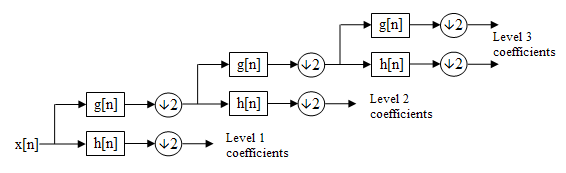
\includegraphics[width=1.0\textwidth]{fig/Wavelets_-_Filter_Bank.png}
    \caption{Cascading}
    \label{fig:filterCascade}
\end{figure}

\subsection{Code \& Results}
Use total number of \(\log_{2}n\) 2x2 orthogonal matrixs as the
filter bank for each layer, which is a (\(\log_{2}n\),2,2) tensor
\(\Phi\).

The optimization problem can be written as follow
\[
    \min_{\Phi}(-\sum_{k=1}^{n}\hat{l}_k^4)
\]

The decomposition function is
\[
    (l,\Phi)\to \hat{l}
\]

So we will obtain a minimum \(\Phi^*\) as the optimal
compression

Then we can send the tensor \(\Phi\) and the reduced
\(\mathring{l}\) to reconstruction.
You can run these \cite[Code]{HaarAugmentedBAT} code to obtain same level results.

\subsubsection{Results}
\begin{figure}[ht!]
    \centering
    \begin{minipage}{0.45\textwidth}
        \centering
        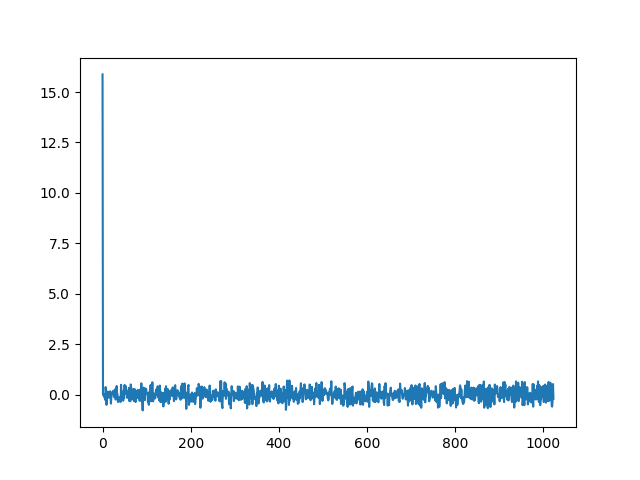
\includegraphics[width=0.9\textwidth]{fig/HaarAugmented1D_freq.png} % first figure itself
        \caption{Haar 2x2 filter bank random input. Compression Rate 0.2568}
        \label{fig:Haar}
    \end{minipage}\hfill
    \begin{minipage}{0.45\textwidth}
        \centering
        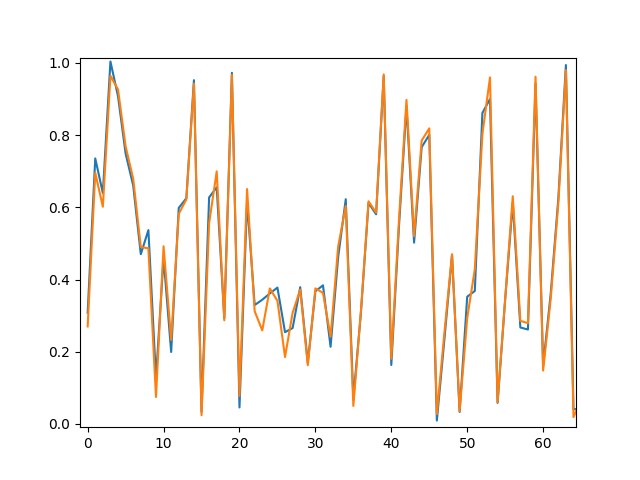
\includegraphics[width=0.9\textwidth]{fig/HaarAugmented1D_rec.png} % second figure itself
        \caption{Haar 2x2 filter bank random input.Total average energy loss 0.0009}
    \end{minipage}
\end{figure}
random sequence would take more information entropy so have a low compress rate.
\begin{figure}[ht!]
    \centering
    \begin{minipage}{0.45\textwidth}
        \centering
        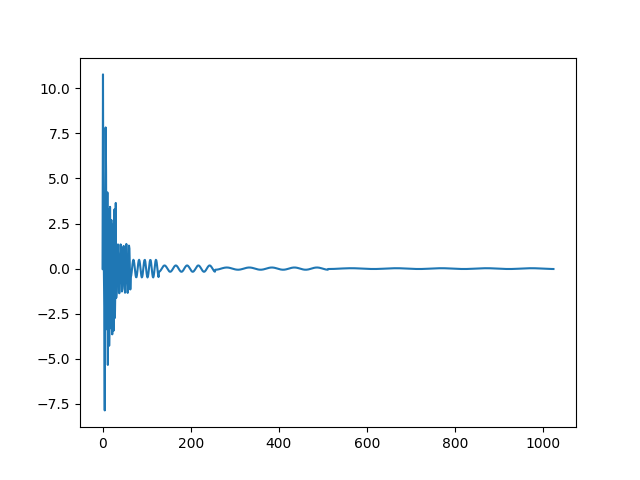
\includegraphics[width=0.9\textwidth]{fig/HaarAugmented1D_sin_freq.png} % first figure itself
        \caption{Haar 2x2 filter bank sin input frequency. Compression Rate 0.9287}
        \label{fig:Haar_sin}
    \end{minipage}\hfill
    \begin{minipage}{0.45\textwidth}
        \centering
        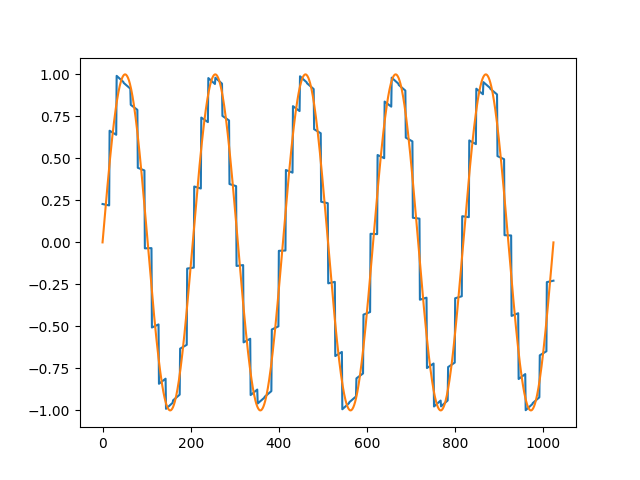
\includegraphics[width=0.9\textwidth]{fig/HaarAugmented1D_sin_rec.png} % second figure itself
        \caption{Haar 2x2 filter bank sin input reconstruction.Total average energy loss 0.0104}
    \end{minipage}
\end{figure}
a smooth signal not have much information entropy, so will have a high compress rate.

\begin{figure}[ht!]
    \centering
    \begin{minipage}{0.45\textwidth}
        \centering
        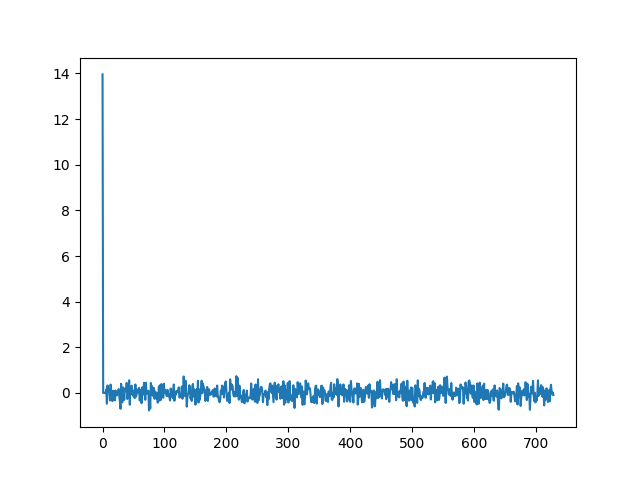
\includegraphics[width=0.9\textwidth]{fig/Haar3Augmented1D_freq.png} % first figure itself
        \caption{Haar 3x3 filter bank random input. Compression Rate 0.1906}
        \label{fig:Haar3}
    \end{minipage}\hfill
    \begin{minipage}{0.45\textwidth}
        \centering
        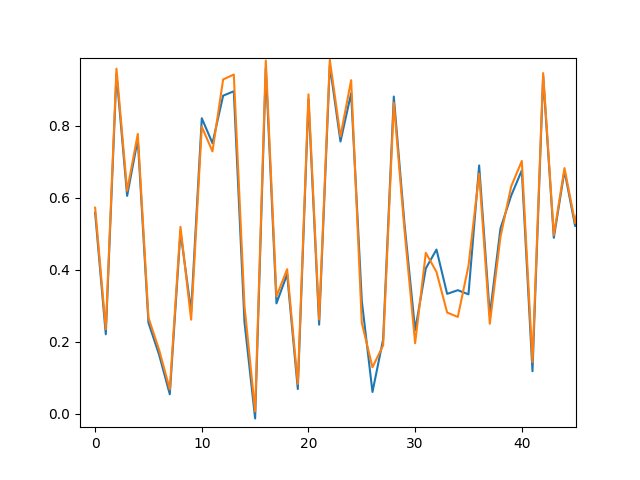
\includegraphics[width=0.9\textwidth]{fig/Haar3Augmented1D_rec.png} % second figure itself
        \caption{Haar 3x3 filter bank random input.Total average energy loss 0.0008}
    \end{minipage}
\end{figure}
\begin{figure}[ht!]
    \centering
    \begin{minipage}{0.45\textwidth}
        \centering
        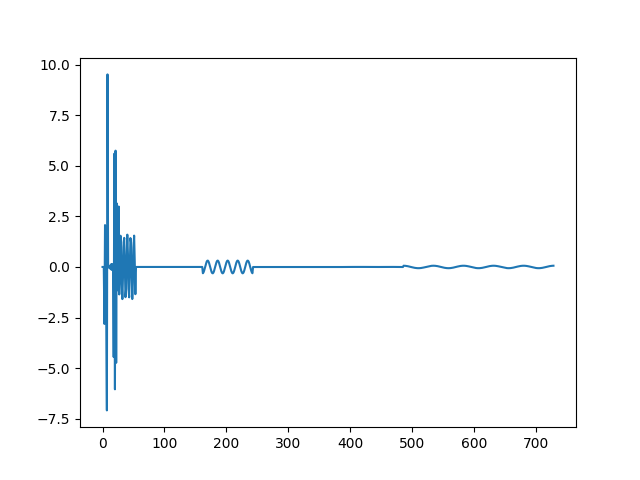
\includegraphics[width=0.9\textwidth]{fig/Haar3Augmented1D_sin_freq.png} % first figure itself
        \caption{Haar 3x3 filter bank sin input frequency. Compression Rate 0.7750}
        \label{fig:Haar3_sin}
    \end{minipage}\hfill
    \begin{minipage}{0.45\textwidth}
        \centering
        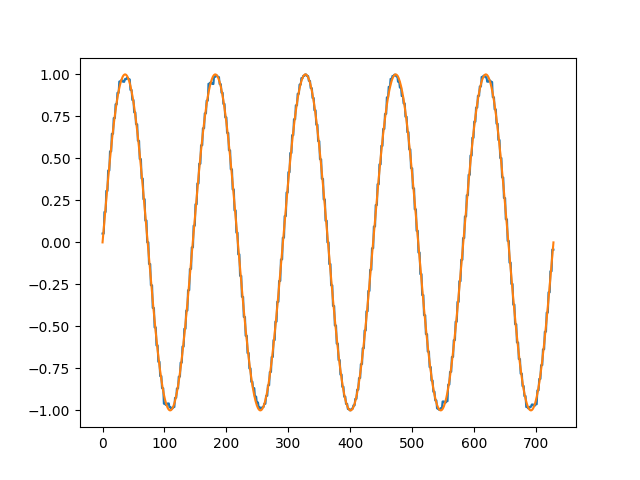
\includegraphics[width=0.9\textwidth]{fig/Haar3Augmented1D_sin_rec.png} % second figure itself
        \caption{Haar 3x3 filter bank sin input reconstruction.Total average energy loss 0.0007}
    \end{minipage}
\end{figure}

% \begin{figure}[ht!]
%     \centering
%     \begin{minipage}{0.45\textwidth}
%         \centering
%         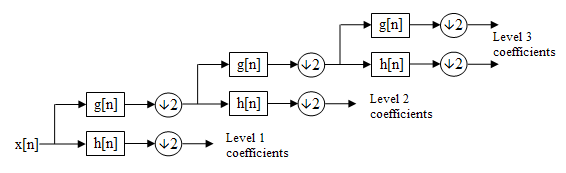
\includegraphics[width=0.9\textwidth]{fig/Wavelets_-_Filter_Bank.png} % first figure itself
%         \caption{sample1 randomly initial position}
%         \label{fig:fig1}
%     \end{minipage}\hfill
%     \begin{minipage}{0.45\textwidth}
%         \centering
%         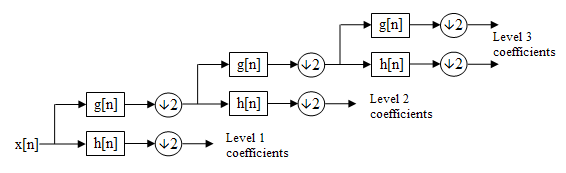
\includegraphics[width=0.9\textwidth]{fig/Wavelets_-_Filter_Bank.png} % second figure itself
%         \caption{sample1 after a period of time}
%     \end{minipage}
% \end{figure}


\section{Fractal Approach}
For a mother wavelet \(\psi(x)\) satisfied
following property.
\[
    \langle\psi,\psi\rangle=1
\]
\[
    \int_{-\infty}^{\infty}\psi(x)dx=0
\]
And the family
\[
    \psi_{j,k}=\sqrt{2^j}\psi(2^j(x-2^{-j}k)) \, j,k\in \mathbb{Z}
\]
For any function satisfied
the following property
\[
    \int_{-\infty}^{\infty}f(x)dx=0
\]
We can decomposed it in to the form
\[
    f=c_{j,k}\psi_{j,k}
\]
And the coefficients can obtained by
the following inner product.
\[
    \langle f,\psi_{j,k}\rangle=c_{j,k}
\]

For a function restricted on
\([0,1]\) we can only use
\[
    \psi_{j,k}=\sqrt{2^j}\psi(2^j(x-2^{-j}k)) \,
    \, k<2^j \, j,k\in \mathbb{N}
\]
To decomposed.

And even more for a discrete function restricted on
\([0,1]\), with \(2^n\) sample points we can only use
\[
    \psi_{j,k}=\sqrt{2^j}\psi(2^j(x-2^{-j}k)) \,
    \, k<2^j\leq2^n \, j,k\in \mathbb{N}
\]
To decomposed.

The inverse process to generate all \(\psi_{j,k}\)
for the discrete case I want to propose a different
approach.

Say I can have a function
\[
    F:\mathbb{R}^2\to\mathbb{R}^2
\]
and a base vector
\[
    [v_0,v_1]
\]
then the next basis would obtain by
the following
\[
    F([v_0,v_1])=[w_0,w_2]
\]
the next basis is
\[
    [w_0,w_1,w_2,w_3]
\]
To keep every iteration to be orthogonal
We need to restrict \(F\)
as following.
\[
    w_1=-\frac{v_0w_0}{v_1}
\]
\[
    w_3=-\frac{v_0w_2}{v_1}
\]
Then every basis need to be nomalized
to fit the property
\[
    \langle\psi,\psi\rangle=1
\]
Then using
\[
    [v_0,v_1]
\]
and \(F\)
we can generate all the basis.

Do the nomal decomposition we will
get coefficients \(c_{j,k}\)
We know \(c_{j,k}c_{j,k}=C\)
If we want all the information
constrain in one coefficients
we need to make
\(c_{j,k}c_{j,k}c_{j,k}c_{j,k}\)
as large as possible.

This is a parameter optimization
problem
\[
    \max_{F,[v_0,v_1]}c_{j,k}c_{j,k}c_{j,k}c_{j,k}
\]

Then we can just transfer \(F\) and \([v_0,v_1]\)




% \subsection{a simple prompt}
% To be more clear of the notations we use,
% we have \(i\in\{1,2,...,10\}=N\)
% And the drones are ignored of its flying
% height, which the position vector can be a
% 2d vector note it as \(\vec{d_i}\)
% And so the velocity and acceleration we denote as
% \(\vec{v_i}=\frac{d\vec{d_i}}{dt}\)
% and
% \(\vec{a_i}=\frac{d\vec{v_i}}{dt}\)
% I want to prompt a \(f\) so that it can form
% a cirle.
% \[
%     \vec{f_i}=m_i(\sum_{\forall k\neq i,\|\vec{d_i}-\vec{d_k}\|\leq R}(\frac{\vec{d_i}-\vec{d_k}}{\|\vec{d_i}-\vec{d_k}\|^3})+(\frac{\vec{d_{t(i)}}-\vec{d_i}}{\|\vec{d_{t(i)}}-\vec{d_i}\|}-v_i))
% \]
% This model is easy to explain, the first term is
% just a inverse square propell force, the second
% term is make the velocity quickly approch a set direction
% the \(t(i)\) is just a randomly choosed target drone
% other than \(i\) that is \(t(i)\in N, t(i)\neq i\)

% This formula can be rewrite without physical term as
% follow.
% \[
%     \vec{a_i}=\sum_{\forall k\neq i,\|\vec{d_i}-\vec{d_k}\|\leq R}(\frac{\vec{d_i}-\vec{d_k}}{\|\vec{d_i}-\vec{d_k}\|^3})+(\frac{\vec{d_{t(i)}}-\vec{d_i}}{\|\vec{d_{t(i)}}-\vec{d_i}\|}-v_i)
% \]
% separately view this is combined by two independent force
% \[
%     (\vec{a_i})_{target}=(\frac{\vec{d_{t(i)}}-\vec{d_i}}{\|\vec{d_{t(i)}}-\vec{d_i}\|}-v_i)
% \]
% \[
%     (\vec{a_i})_{propell}=\sum_{\forall k\neq i,\|\vec{d_i}-\vec{d_k}\|\leq R}(\frac{\vec{d_i}-\vec{d_k}}{\|\vec{d_i}-\vec{d_k}\|^3})
% \]

% \subsection{a simple prompt:simulation}
% \subsubsection{Four drone case:derivation}
% This case just choose \(N=\{1,2,3,4\}\)
% and don't allow \(t(t(i))=i\)
% which definitely form a three element loop and
% a dangling drone.

% We have a (4,2)-tensor \(\vec{d_i}\)
% and two other (4,2)-tensor \(\vec{v_i}\)
% and \(\vec{a_i}\)
% The initial points are randomly choosed
% in Uniformly \([0,1]\times[0,1]\)

% choose a time increment \(dt\)
% and the simulation update formula is simple to write

% just as follow
% \[\begin{bmatrix}
%         \vec{{d_{n+1}}_i} \\
%         \vec{{v_{n+1}}_i}
%     \end{bmatrix}=
%     \begin{bmatrix}
%         \vec{{d_{n}}_i}+\vec{{v_n}_i}dt \\
%         \vec{{v_{n}}_i}+(\sum_{\forall k\neq i,\|\vec{{d_n}_i}-\vec{{d_n}_k}\|\leq R}(\frac{\vec{{d_n}_i}-\vec{{d_n}_k}}{\|\vec{{d_n}_i}-\vec{{d_n}_k}\|^3})+(\frac{\vec{{d_n}_{t(i)}}-\vec{{d_n}_i}}{\|\vec{{d_n}_{t(i)}}-\vec{{d_n}_i}\|}-{v_n}_i))dt
%     \end{bmatrix}
% \]
% simple Euler method.

% \subsubsection{Four drone case:code \& result}
% the computational code are \cite[FourDroneCase]{FourDroneCase} .
% the results are shown by the following pictrues which
% generated by the code.
% The video are \cite[sample1-video]{sample1-video}
% and \cite[sample2-video]{sample2-video}
% and more other in the same folder on github.
% \begin{figure}[ht!]
%     \centering
%     \begin{minipage}{0.45\textwidth}
%         \centering
%         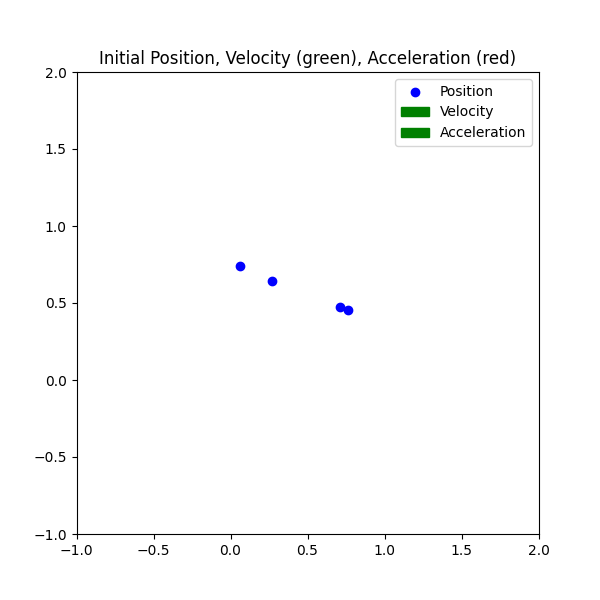
\includegraphics[width=0.9\textwidth]{fig/sample1/dd.png} % first figure itself
%         \caption{sample1 randomly initial position}
%         \label{fig:fig1}
%     \end{minipage}\hfill
%     \begin{minipage}{0.45\textwidth}
%         \centering
%         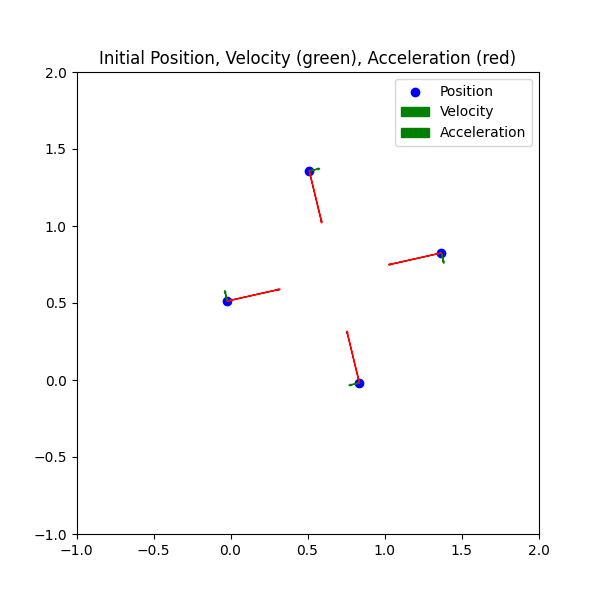
\includegraphics[width=0.9\textwidth]{fig/sample1/dd_18254.png} % second figure itself
%         \caption{sample1 after a period of time}
%     \end{minipage}
% \end{figure}
% \begin{figure}[ht!]
%     \centering
%     \begin{minipage}{0.45\textwidth}
%         \centering
%         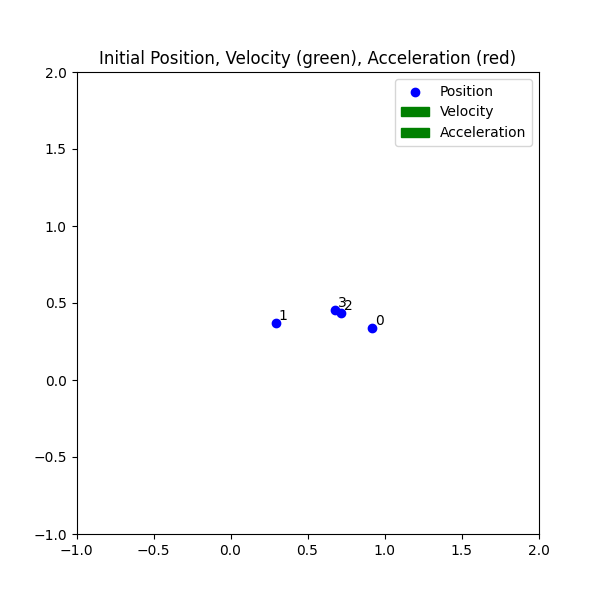
\includegraphics[width=0.9\textwidth]{fig/sample2/dd.png} % first figure itself
%         \caption{sample1 randomly initial position}
%         \label{fig:fig2}
%     \end{minipage}\hfill
%     \begin{minipage}{0.45\textwidth}
%         \centering
%         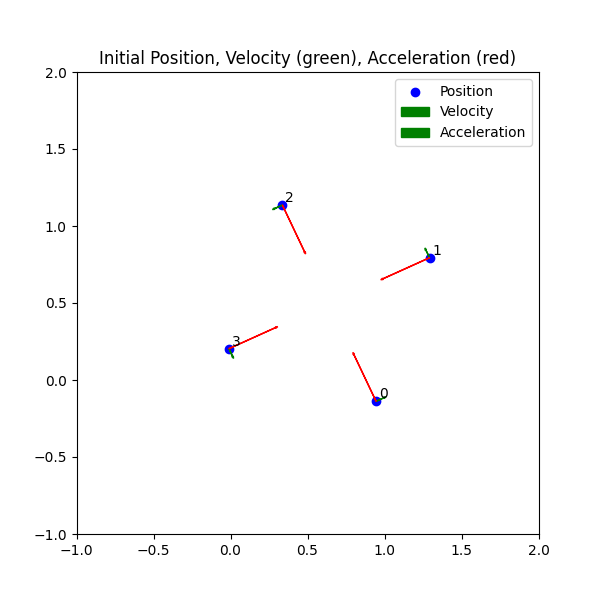
\includegraphics[width=0.9\textwidth]{fig/sample2/dd_18993.png} % second figure itself
%         \caption{sample2 after a period of time}
%     \end{minipage}
% \end{figure}

% \subsubsection{Ten drone case:derivation}
% undergoing

% \subsubsection{Ten drone case:result}
% undergoing

% \subsection{some analysis why it will have a stability property}
% \subsubsection{the terminate radius R}
% undergoing

% \subsubsection{the terminate center O}
% undergoing

% \subsubsection{graph theory part}
% The \(t(i)\) forms a graph which have \(n\) points
% and \(n\) oriented edges, this forms a tree with a extra
% edges, and this case It will obviously form a Unicyclic Graph.

% Which is a tree if we treat all the point on the
% loop as the same point.

% \subsection{target distance method}
% undergoing

% \subsection{target distance method:simulation}
% undergoing


% \section{Zinan Su's approach}
% \subsection{notations \& equations}
% safe collide radius is \(d_s\)
% \[
%     \sigma=2d_s
% \]
% \(NUM\) is the total number of the drones.
% And then we want the following dynamic system
% \[\begin{bmatrix}
%         \frac{d\vec{p_i}}{dt} \\
%         \frac{d\vec{v_i}}{dt}
%     \end{bmatrix}=
%     \begin{bmatrix}
%         \vec{v_i} \\
%         \vec{a_i}
%     \end{bmatrix}
% \]
% circle origin is a function
% \[
%     c=\frac{1}{NUM}\sum_{k=1}^{NUM}p_k
% \]
% Four constants.
% \[
%     k_p=
% \]
% \[
%     k_d=
% \]
% \[
%     k_v=
% \]
% \[
%     k_r=
% \]
% \[
%     R^*=\frac{1}{NUM}\sum_{k=1}^{NUM}p_k(0)-c(0)
% \]
% \[
%     v_d=\frac{1}{NUM}\sum_{k=1}^{NUM}\|v_k(0)\|
% \]
% and
% \[
%     r_i=p_i-c
% \]
% \[
%     d_i=\|r_i\|
% \]
% \[
%     \hat{r_i}=\frac{r_i}{d_i}
% \]
% \[
%     \hat{\theta_i}=\mathbb{M}_\theta r_i
% \]
% \[
%     \mathbb{M}_\theta=
%     \begin{bmatrix}
%         0  & 1 \\
%         -1 & 0
%     \end{bmatrix}
% \]
% \[
%     {v_{i}}_{\parallel}=\hat{r_i}\cdot v_i
% \]
% \[
%     {v_{i}}_{\perp}=\hat{\theta_i}\cdot v_i
% \]
% \[
%     U(r)=k_re^{-\frac{r}{2\sigma^2}}
% \]
% \[
%     U_{ij}=U(\|p_i-p_j\|)
% \]
% \[
%     \vec{u_i}_1=[-k_p(d_i-R^*)-k_d{v_{i}}_{\parallel}]\hat{r_i}
% \]
% \[
%     \vec{u_i}_2=[-k_v({v_{i}}_{\perp}-v_d)]\hat{\theta_i}
% \]
% \[
%     \vec{u_i}_3=\sum_{\forall k\neq i}(-\nabla_{p_i}U_{ij})
% \]
% \[
%     \vec{u_i}=\vec{u_i}_1+\vec{u_i}_2+\vec{u_i}_3
% \]




\bibliographystyle{plain}  % or another style like unsrt, IEEEtran, etc.
\bibliography{references}  % references.bib is the file name

\end{document}
